\section{Frequency mode 01}
\label{FM01}

\subsection{Spectra}
\label{FM01:spectra}

\begin{figure}[ht]
    \centering
    \begin{subfigure}[b]{0.9545\textwidth}
        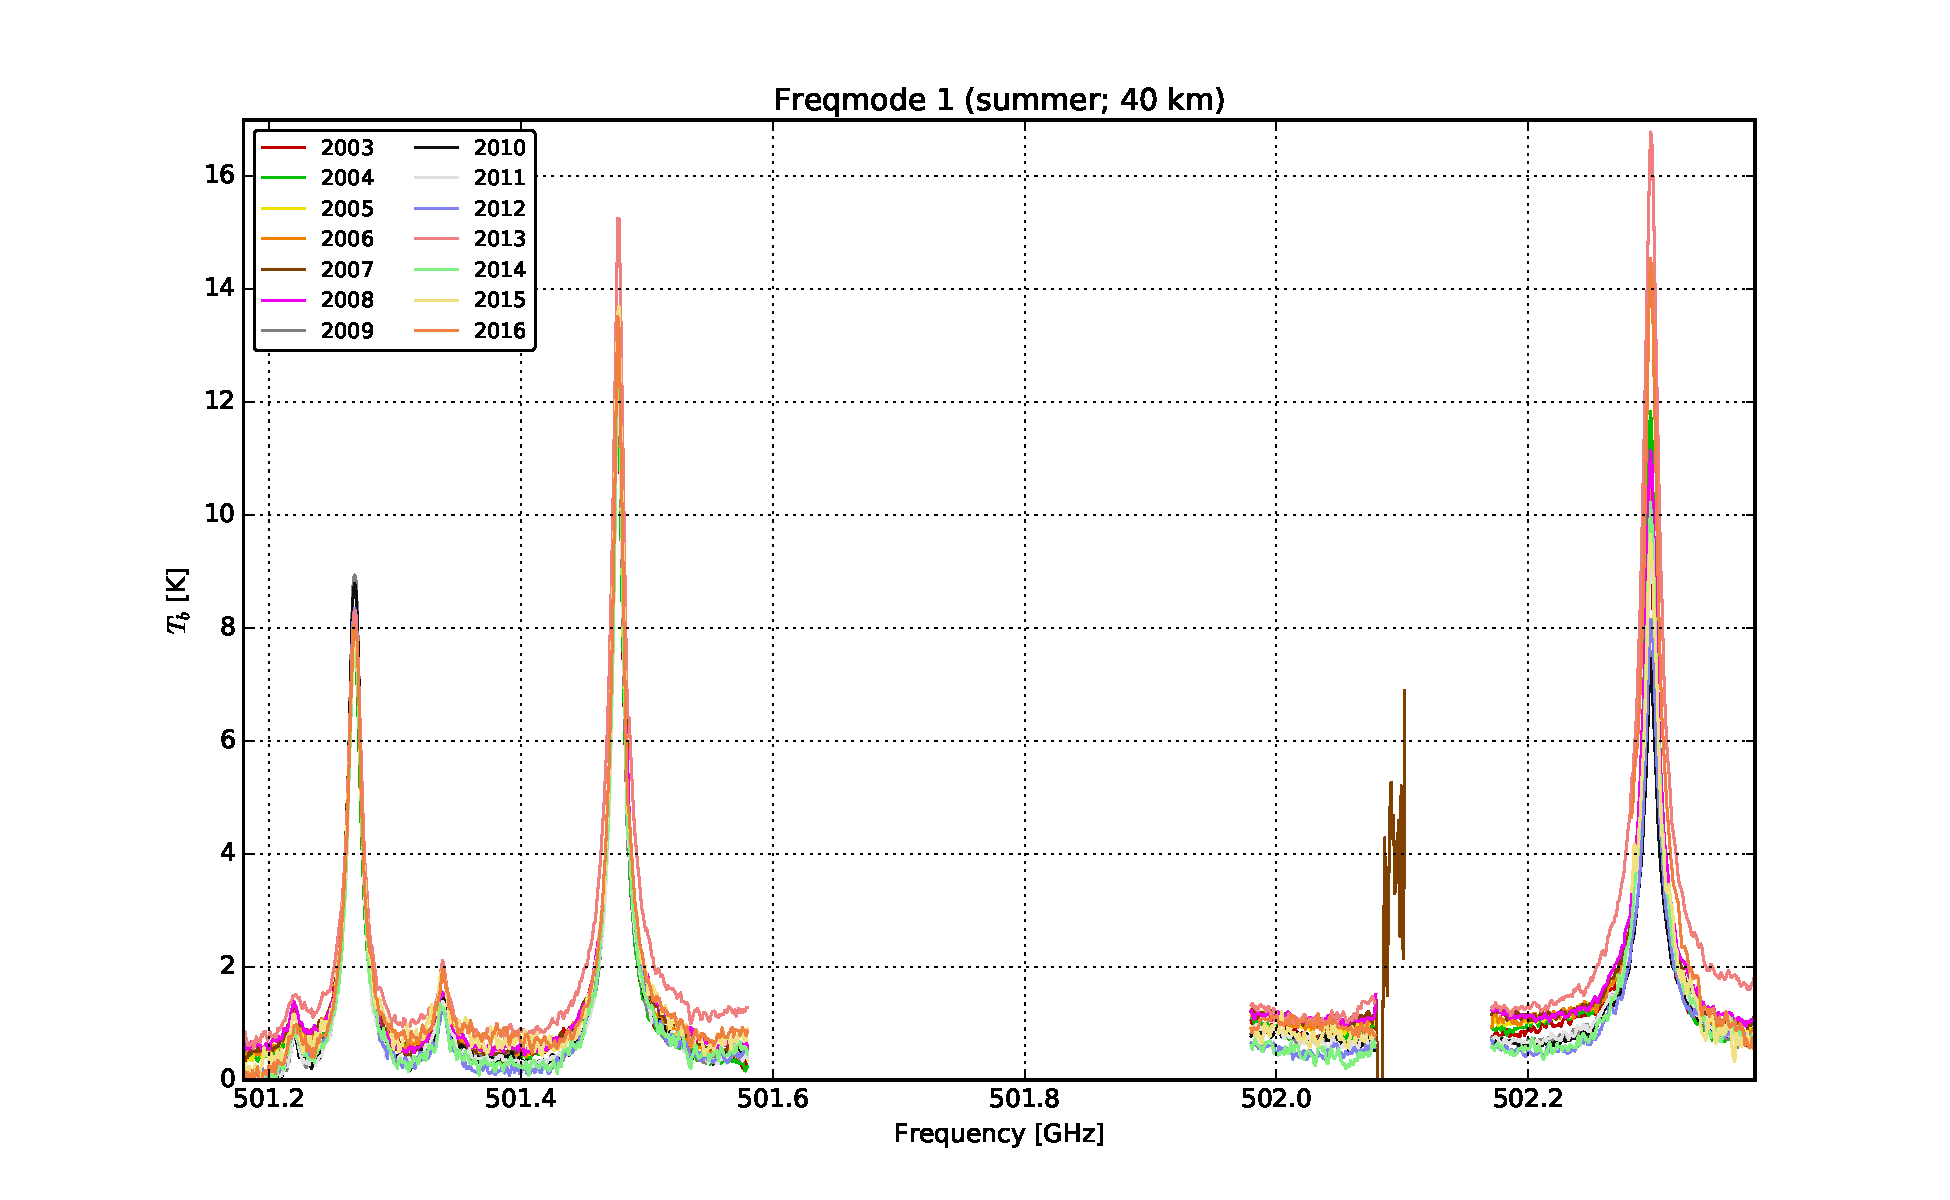
\includegraphics[width=\textwidth]{spectra/fm_01_spectra_summer}
        \caption{summer}\label{fig:spectra:01:summer}
    \end{subfigure}
    \begin{subfigure}[b]{0.9545\textwidth}
        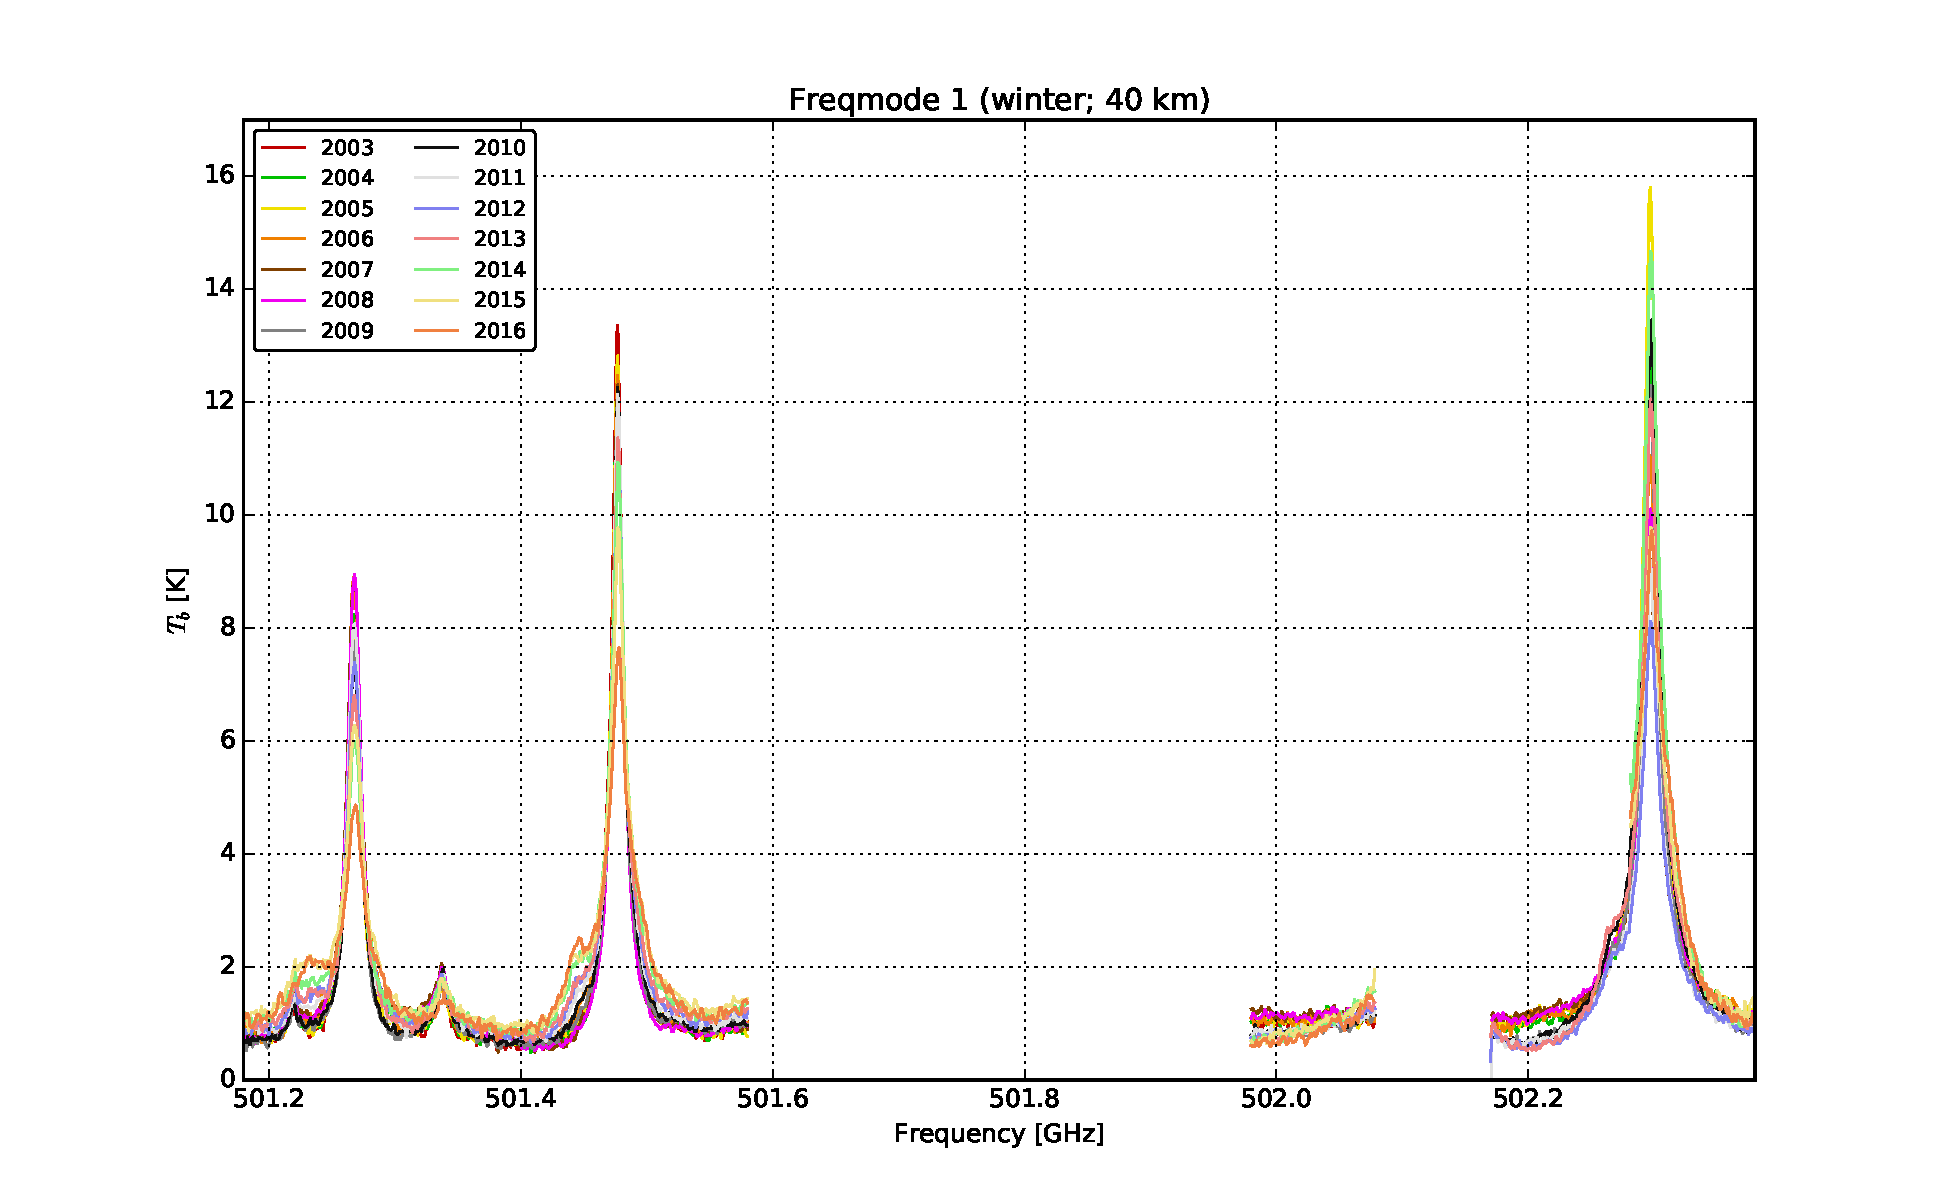
\includegraphics[width=\textwidth]{spectra/fm_01_spectra_winter}
        \caption{winter}\label{fig:spectra:01:winter}
    \end{subfigure}
    \caption{Annual median spectra for FM~01 for altitude interval 35--45~km at
        equatorial latitudes. The unhealthy sub-bands~3 and~7 are between
        $\sim502.08$ and~$502.28\,\mathrm{GHz}$.
        }\label{fig:spectra:01}
\end{figure}

\begin{figure}[ht]
    \centering
    \begin{subfigure}[b]{0.9545\textwidth}
        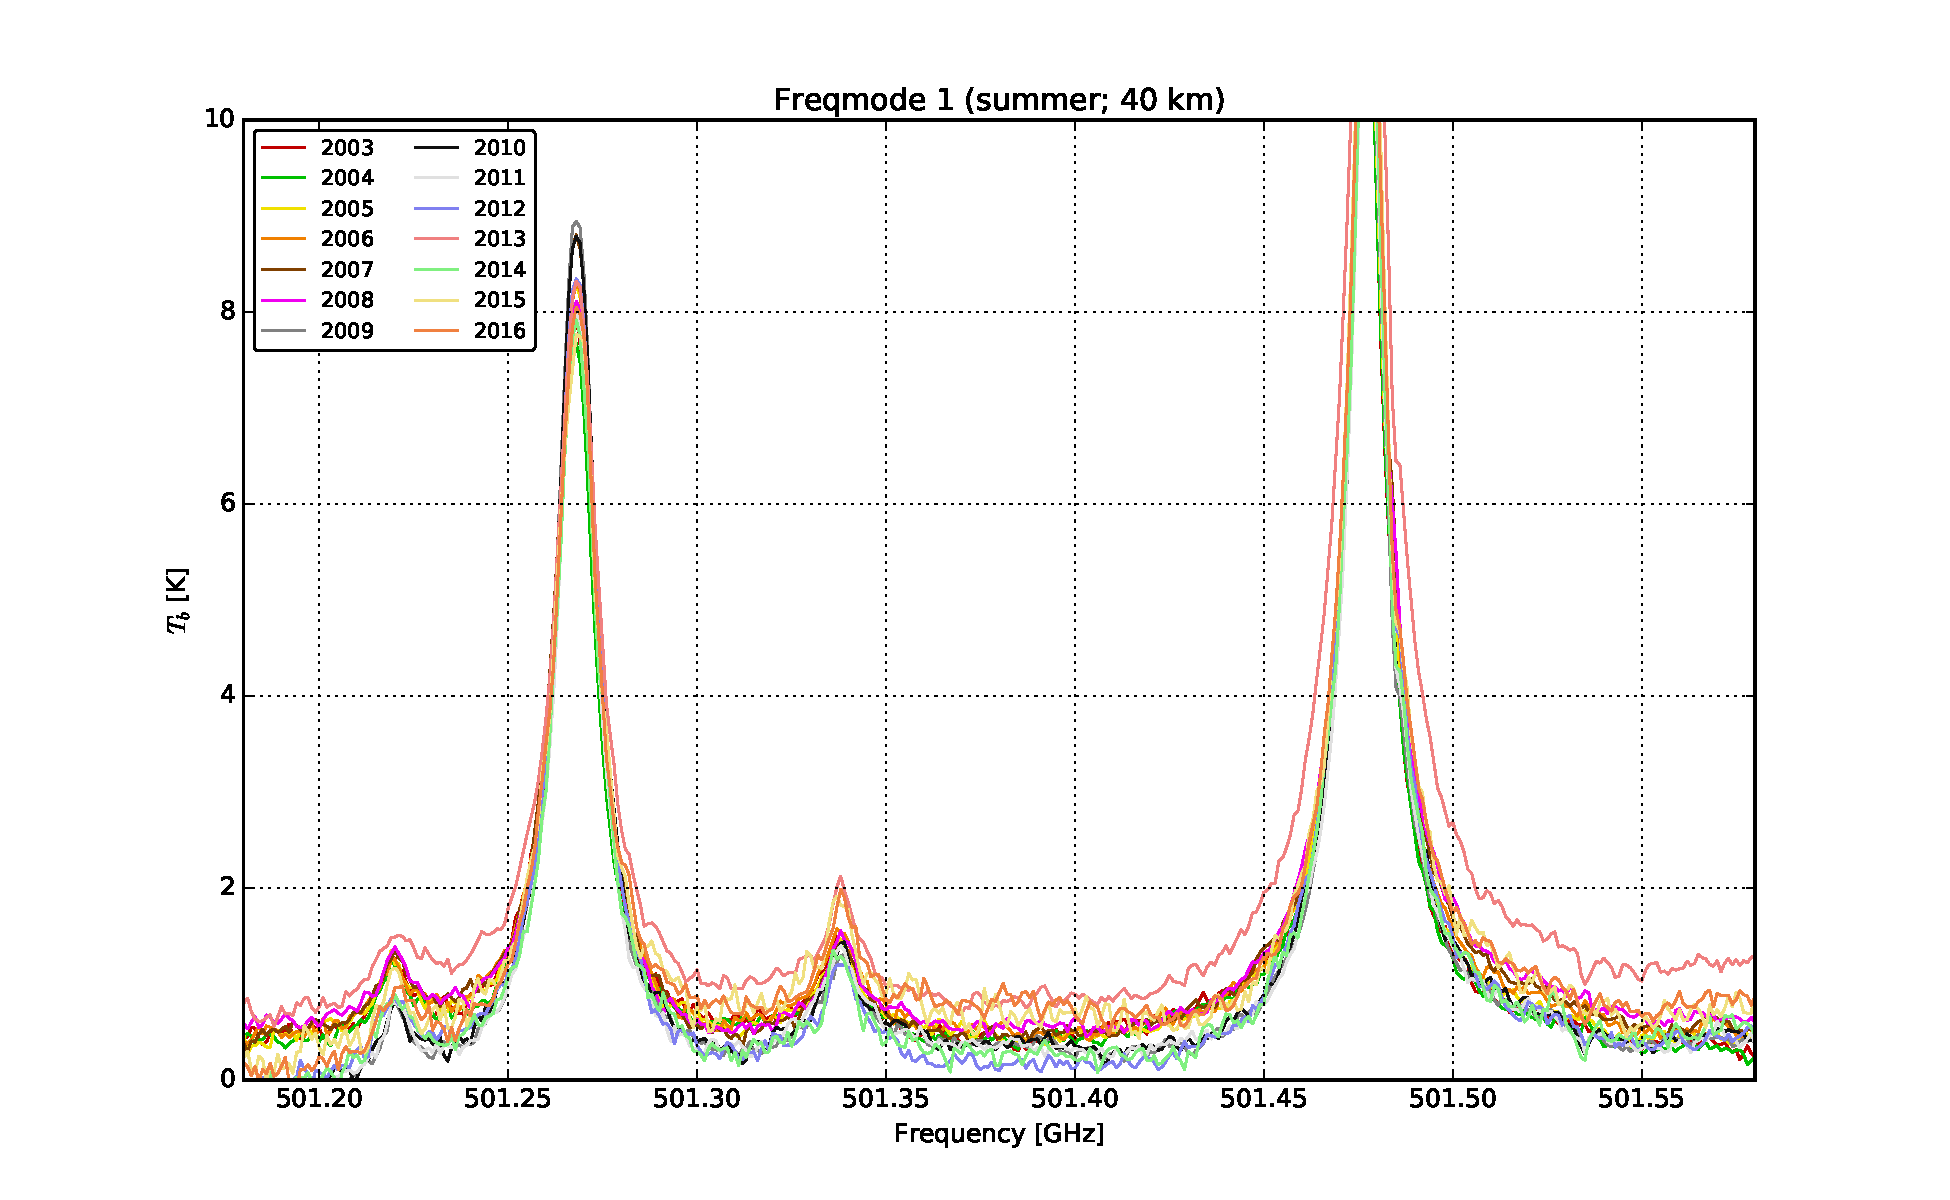
\includegraphics[width=\textwidth]{spectra/fm_01_spectra_summer_zoom_40km}
        \caption{summer}\label{fig:spectra:01:summer:closeup}
    \end{subfigure}
    \begin{subfigure}[b]{0.9545\textwidth}
        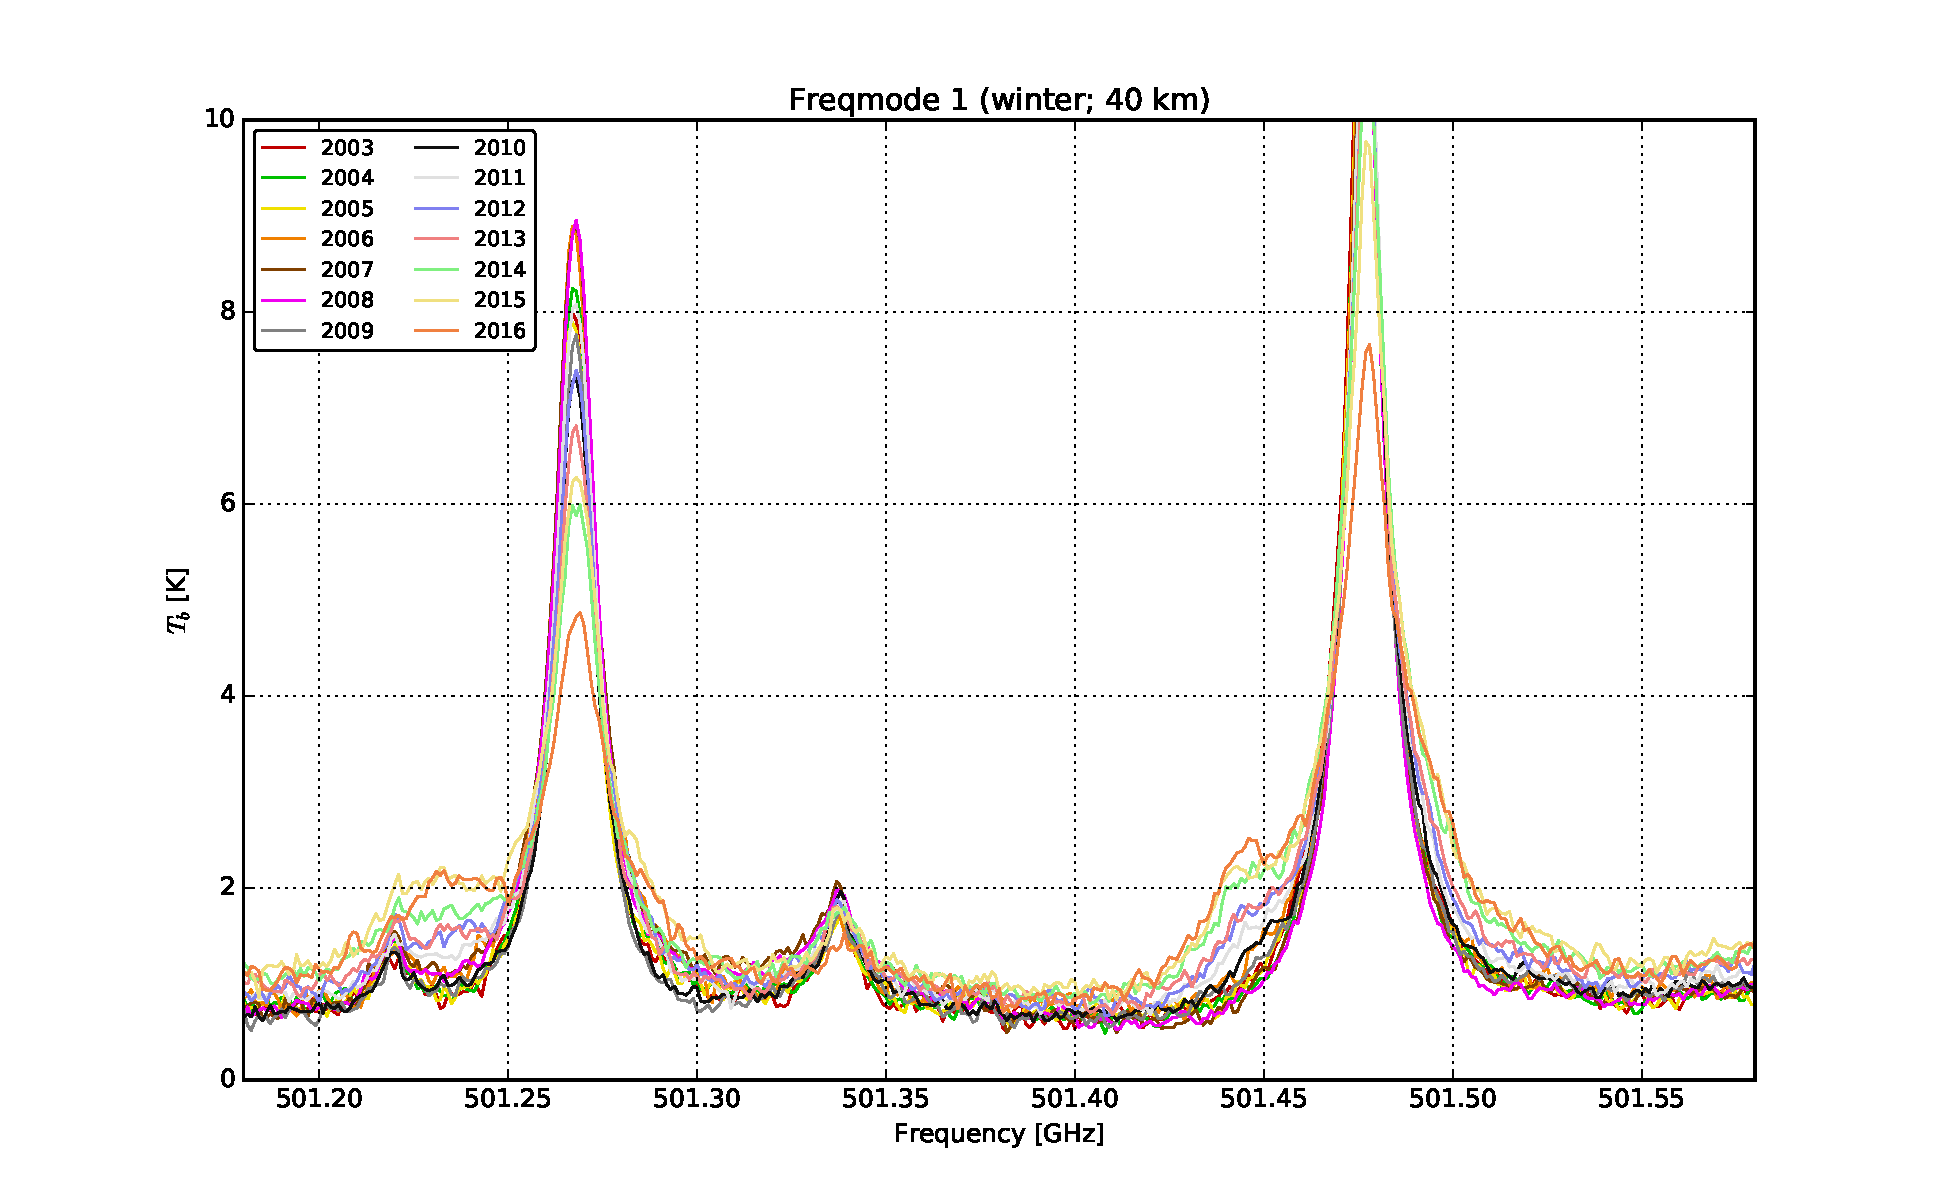
\includegraphics[width=\textwidth]{spectra/fm_01_spectra_winter_zoom_40km}
        \caption{winter}\label{fig:spectra:01:winter:closeup}
    \end{subfigure}
    \caption{Close-up of the annual median spectra for FM~01 for altitude
        interval 35--45~km at equatorial latitudes.
        }\label{fig:spectra:01:closeup}
\end{figure}

\noindent
Yearly median spectra for summer and winter at $\sim40\,\mathrm{km}$ are shown
in Fig.~\ref{fig:spectra:01}.  These and the close-ups seen in
Fig.~\ref{fig:spectra:01:closeup} show that the spectra seem to fall in two
categories, depending on whether they were retrieved before or after 2009, with
spectra retrieved during later years being clustered at a lower baseline
temperature.  This is most evident for the spectra from the summer, when the
sattelite is colder.  Also evident, in particular in the close-ups, is that
that the intensity of the median spectra of the main peaks has been
redistributed to lower frequencies during the later years, possibly due to a
shift in the frequency calibration or in the retrieval itself.  Both of these
effects are discussed below in more detail in Sec.~\ref{FM01:baseline}
and~\ref{FM01:leftwings} respectively.


\subsection{Sideband leakage}
\label{FM01:sbl}
In FM~1 there are two sideband peaks to the right of the main band peak at
$503.3\,\mathrm{GHz}$, but these are note distinct in the spectra show in
Fig.~\ref{fig:spectra:01}.  Furthermore, the fact that these peaks are close
together near the edge of the spectra makes it difficult to extract an
approximate main band baseline to subtract from the peaks such as they are.  It
is therefore very difficult to draw any conclusions as to the long term trends
of the sideband leakage for this mode, but a rough very rough estimate would be
$\sim3$--$7$\%.  A slight tendency to increase over time can be discerned if
one looks closely and squints, but this may be attributed to confirmation bias
on the part of the investigator and should be regarded as speculation at this
point.


\subsection{Seasonality}
\label{FM01:seasonality}

\begin{figure}[ht]
    \centering
    \begin{subfigure}[b]{0.9545\textwidth}
        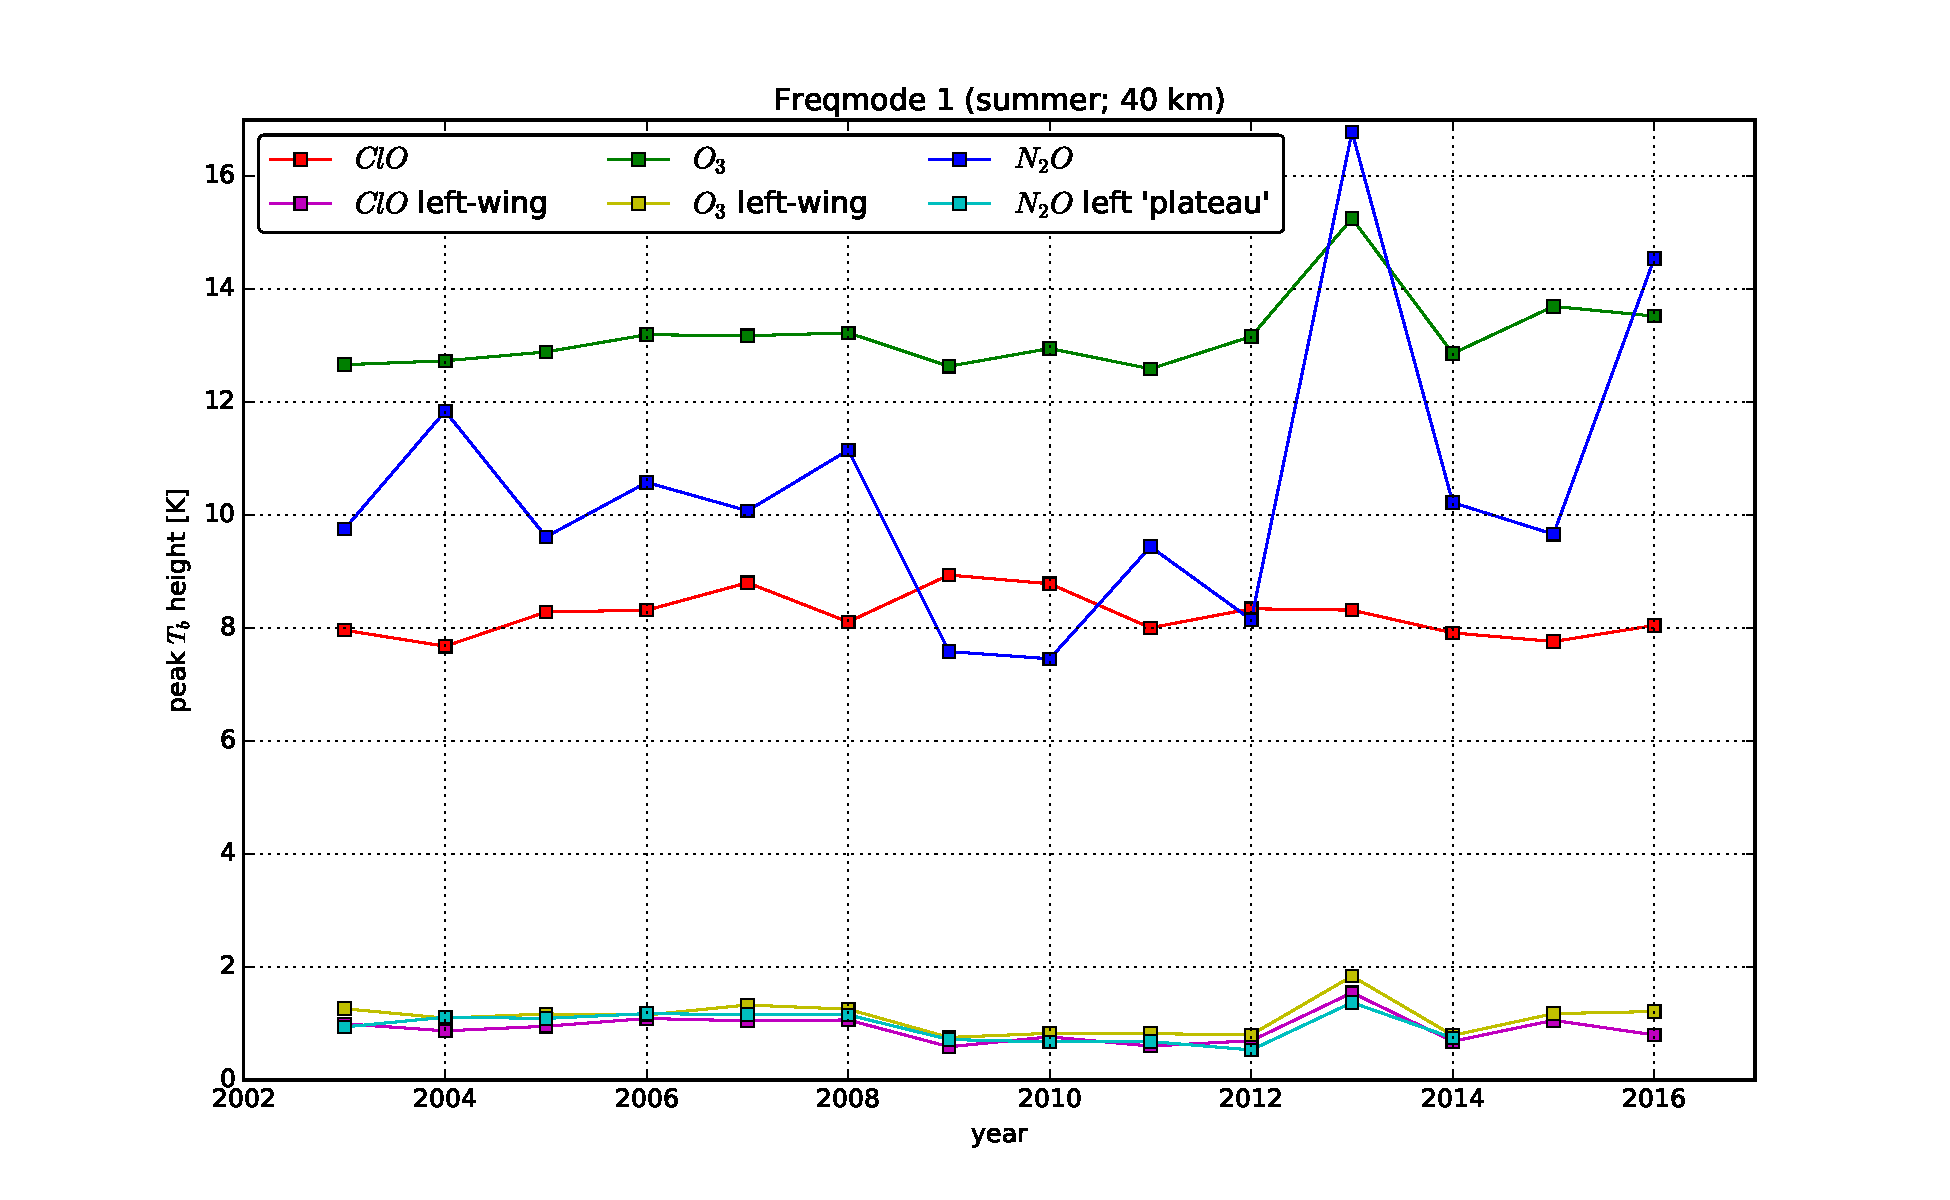
\includegraphics[width=\textwidth]{peaks/fm_01_peaks_summer}
        \caption{summer}\label{fig:peaks:01:summer}
    \end{subfigure}
    \begin{subfigure}[b]{0.9545\textwidth}
        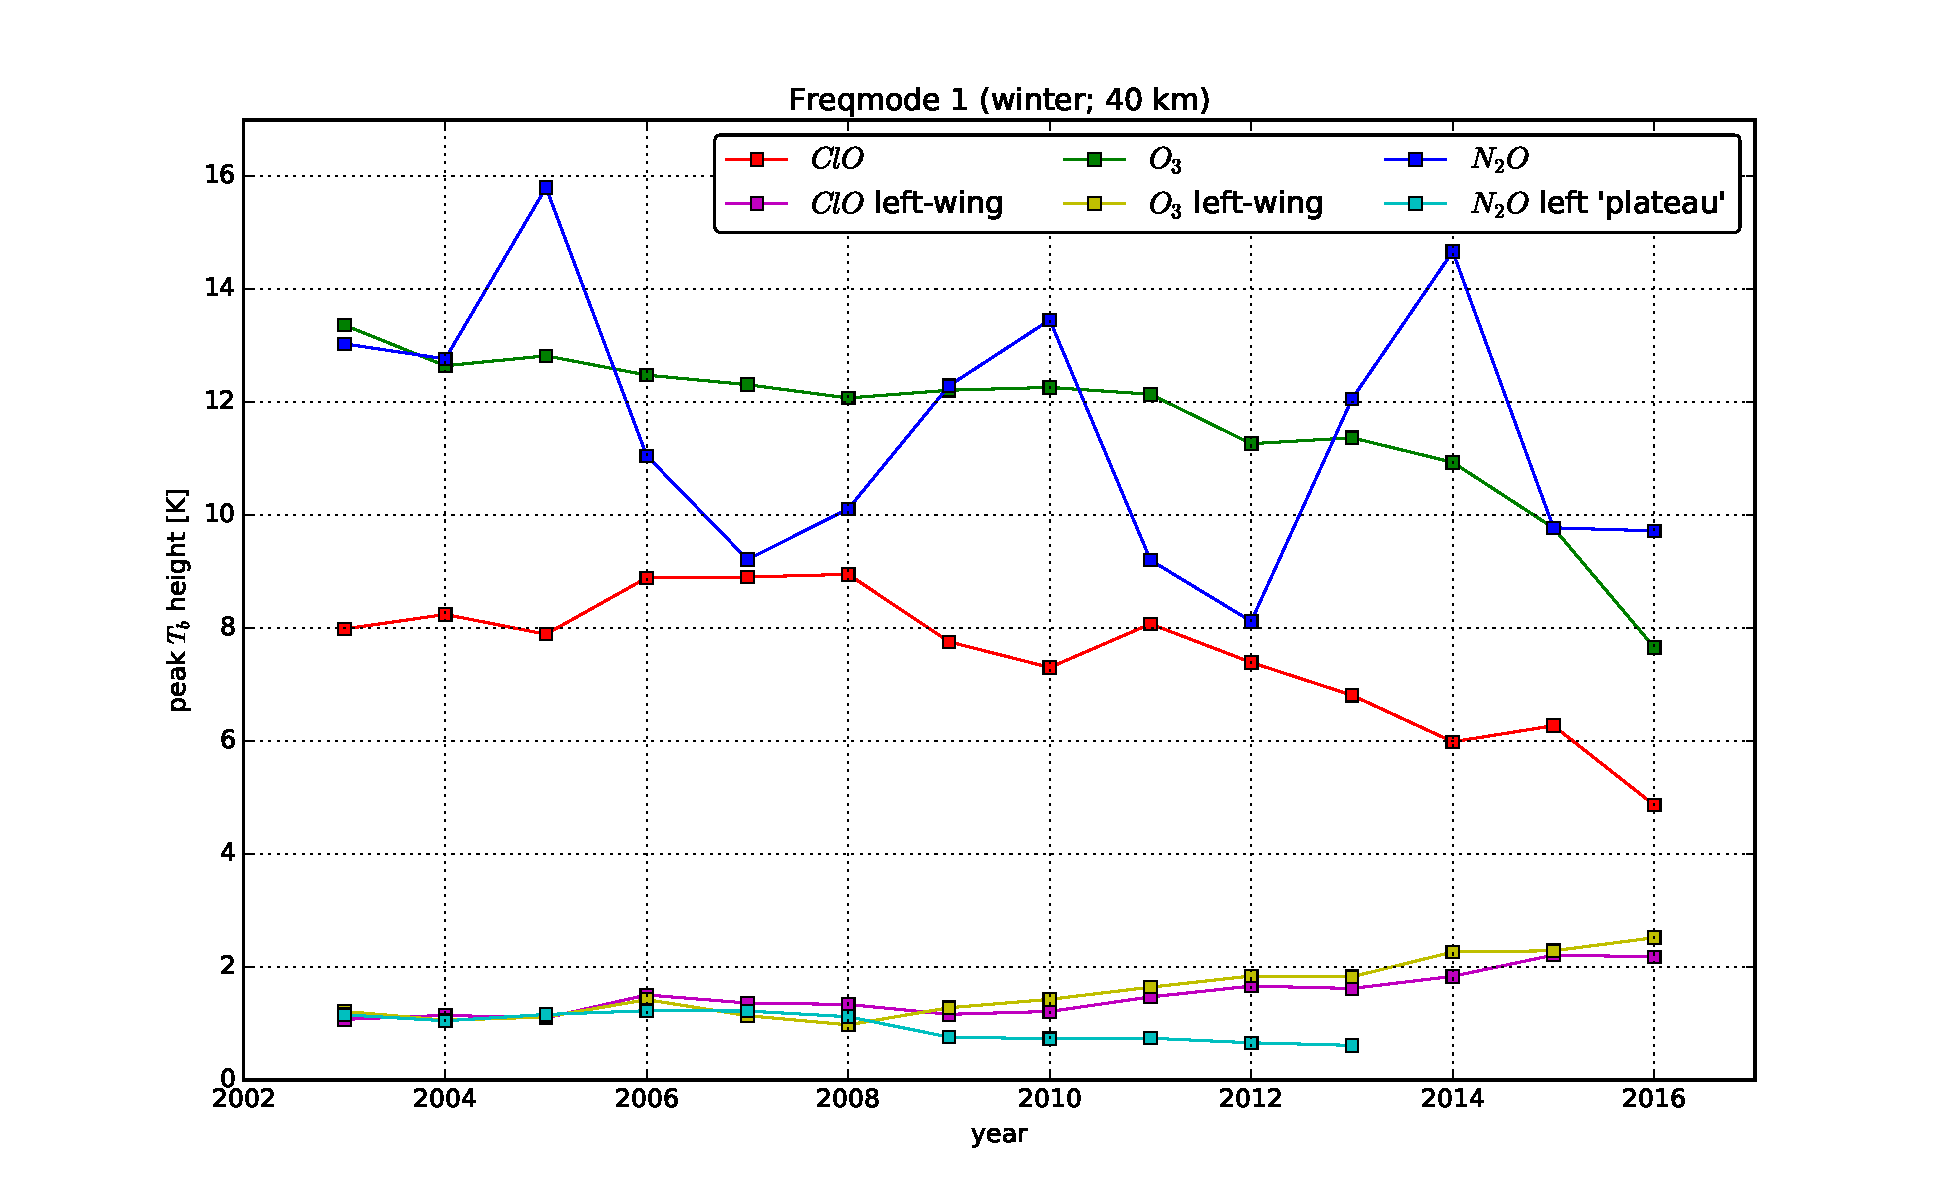
\includegraphics[width=\textwidth]{peaks/fm_01_peaks_winter}
        \caption{winter}\label{fig:peaks:01:winter}
    \end{subfigure}
    \caption{Annual median peak values for FM~01 for altitude interval
        35--45~km at equatorial latitudes.  Values extracted for the left
        \chem{ClO} peak at~$\sim551.28\,\mathrm{GHz}$, the \chem{O_3} peak
        at~$\sim551.49\,\mathrm{GHz}$, and the right \chem{N_2O} peak
        at~$\sim552.32\,\mathrm{GHz}$, in Fig.~\ref{fig:spectra:01}.  The
        ``wings'' to the left of the \chem{ClO} and \chem{O_3} peaks, and the
        ``baseline'' at~$\sim502.2\,\mathrm{GHz}$ were also estimated.
        }\label{fig:peaks:01}
\end{figure}

\noindent
Fig.~\ref{fig:peaks:01:summer} shows that during the summers the results for
the \chem{ClO} and \chem{O_3}~peaks vary little (the exception being 2013,
when the general levels appear to be higher, as seen in
Fig.~\ref{fig:spectra:01:summer}).  The \chem{N_2O}~peak, on the other hand,
varies quite a lot, but this can likely be attributed to natural annual
variations.  In contrast, Fig.~\ref{fig:peaks:01:winter} shows decreasing
tendencies for both \chem{ClO} and \chem{O_3} after 2008 or 2009, and a
similar tendency can perhaps be discerned for \chem{N_2O} as well.

The trends of the main peaks correlate with the trends for of the ``wings''.
The wings show little or no increase for the summers, but a clear increase
during the winters after 2008, correlated with a decrease of the same relative
magnitude for the corresponding \chem{ClO} and \chem{O_3}~peaks.  This is
discussed in Sec.~\ref{FM01:leftwings} below.

In addition to the showing the trend of the wings, the baseline left of the
\chem{N_2O} peak has been extracted.  This is discussed in
Sec.~\ref{FM01:baseline} below.


\subsection{Change of ``baseline'' for later years}
\label{FM01:baseline}
As can bee seen in Fig.~\ref{fig:peaks:01}, the baseline before 2009 fluctuates
around $\sim1$~K, whereas after 2009 it is clustered instead around $\sim0.5$~K
for both summer and winter (2013 again being an exception).  This clustering
can also be seen in Fig.~\ref{fig:spectra:02}.  The same change is observed for
FM~02, see Sec.~\ref{FM02:baseline}.  Currently there is no satisfactory
explanation for this, though it may be related to the overall temperature of
the satellite, see~\ref{sec:Tcal} for details.


\subsection{Left-wing splitters}
\label{FM01:leftwings}
The peaks in FM~01 are plagued by a strange malady that first manifested itself
as ``wings'' on the left side of the main band peaks.  All three main peaks are
affected, but it is most clearly seen for the \chem{ClO} and \chem{O_3} peaks
shown in Fig.~\ref{fig:spectra:01:closeup}.  The phenomenon appears to have
started in 2009 and is not observed during the summer, when the satellite is
colder.  The problem has been growing worse over the years, manifesting itself
almost as ghost-peaks rather than wings in 2014--2016.  As noted above and seen
in Figs.~\ref{fig:spectra:01:closeup} and~\ref{fig:peaks:01}, the phenomenon is
only evident during the winter, which indicates that it might be temperature
dependent since during the winter the satellite is warmer (see~\ref{sec:Tcal}).
The trend also correlates with an increased receiver temperature, as seen
in~\ref{fig:trec}.

From Fig.~\ref{fig:spectra:01:closeup} it is clear that the effect assymetric
and therefore not a simple broadening of the lines.  Rather it appears that
spectral intensity has been moved from the peak values and deposited over an
interval $\sim50\,\mathrm{MHz}$ beginning below the peak.  In particular for
later years, the effect seems to also extend a few $\mathrm{MHz}$ above the
peak.  Since the figure shows median spectra, this is consistent with a portion
of spectra having been shifted to to lower frequencies, misplacing the peak.
This is also consistent with Fig.~\ref{fig:peaks:01:winter}, where it can be
seen that the rise in the wings are correlated with a fall in the peak values
of roughly the same order.  Though the notion that a portion of the spectra
have somehow been shifted seems a likely explanation, so far it has not been
confirmed when looking at individual spectra.  It should be more thoroughly
investigated before being ruled out.  One route ahead might be to look at daily
spectra, though if the phenomenon is similar to that of the \chem{CO} modes
(FMs~14, 22 and~24) the shift likely occurs during the beginning of a
measurement period, which might make it hard to spot using this
method.\todo{ref to CO mode freq shifts when written}

As seen in Fig.~\ref{fig:spectra:01}, the wings are not as evident around the
\chem{N_2O} at $\sim502.3\,\mathrm{GHz}$, which is likely due in part to the
afflicted region being in the unhealthy subband~7, which is missing from later
years.  Looking at the three main peaks in Fig.~\ref{fig:spectra:01:winter},
however, it appears that the ``shift'' may be more pronounced for lower
frequencies, with the left-most \chem{ClO} peak showing the largest down-shift
and the right-most \chem{N_2O} peak showing the smallest.  This frequency
dependence of the effect is speculative at this point, but might deserve
further investigation.
